\documentclass[
oneside,			% para impressão em recto e verso. Oposto a oneside
% -- opções da classe abntex2 --
chapter=TITLE,		% títulos de capítulos convertidos em letras maiúsculas
section=TITLE,		% títulos de seções convertidos em letras maiúsculas
%subsection=TITLE,	% títulos de subseções convertidos em letras maiúsculas
%subsubsection=TITLE,% títulos de subsubseções convertidos em letras maiúsculas
]{settings/utfpr-tcc}

%=======================================
% Setar configurações
%---------------------------------------
% REFERÊNCIAS------------------------------------------------------------------
\usepackage[%
alf,
abnt-emphasize=bf,
bibjustif,
recuo=0cm,
abnt-url-package=url,       % Utiliza o pacote url
abnt-refinfo=yes,           % Utiliza o estilo bibliográfico abnt-refinfo
abnt-etal-cite=3,
abnt-etal-list=3,
abnt-thesis-year=final
]{abntex2cite}                  % Configura as citações bibliográficas conforme a norma ABNT

% PACOTES----------------------------------------------------------------------
\usepackage[utf8]{inputenc}                                 % Codificação do documento
\usepackage[T1]{fontenc}                                    % Seleção de código de fonte
\usepackage{booktabs}                                       % Réguas horizontais em tabelas
\usepackage{color, colortbl}                                % Controle das cores
\usepackage{float}                                          % Necessário para tabelas/figuras em ambiente multi-colunas
\usepackage{graphicx}                                       % Inclusão de gráficos e figuras
\usepackage{icomma}                                         % Uso de vírgulas em expressões matemáticas
\usepackage{indentfirst}                                    % Indenta o primeiro parágrafo de cada seção
\usepackage{microtype}                                      % Melhora a justificação do documento
\usepackage{multirow, array}                                % Permite tabelas com múltiplas linhas e colunas
\usepackage{subeqnarray}                                    % Permite subnumeração de equações
\usepackage{lastpage}                                       % Para encontrar última página do documento
\usepackage{verbatim}                                       % Permite apresentar texto tal como escrito no documento, ainda que sejam comandos Latex
\usepackage{amsfonts, amssymb, amsmath}                     % Fontes e símbolos matemáticos
\usepackage[algoruled, portuguese]{algorithm2e}             % Permite escrever algoritmos em português
%\usepackage[scaled]{helvet}                                % Usa a fonte Helvetica
\usepackage{times}                                          % Usa a fonte Times
%\usepackage{palatino}                                      % Usa a fonte Palatino
%\usepackage{lmodern}                                       % Usa a fonte Latin Modern
\usepackage[bottom]{footmisc}                               % Mantém as notas de rodapé sempre na mesma posição
\usepackage{ae, aecompl}                                    % Fontes de alta qualidade
\usepackage{latexsym}                                       % Símbolos matemáticos
\usepackage{lscape}                                         % Permite páginas em modo "paisagem"
%\usepackage{picinpar}                                      % Dispor imagens em parágrafos
%\usepackage{scalefnt}                                      % Permite redimensionar tamanho da fonte
\usepackage{subfig}                                         % Posicionamento de figuras
%\usepackage{upgreek}                                       % Fonte letras gregas
\usepackage[siunitx, american]{circuitikz}                                     % Desenhar circuitos
%\usepackage{tikz}                                     	    % Desenhar circuitos
\usepackage{settings/exercise-list}

% Redefine a fonte para uma fonte similar a Arial (fonte Helvetica)
\renewcommand*\familydefault{\sfdefault}

% CONFIGURAÇÕES DE APARÊNCIA DO PDF FINAL--------------------------------------
\makeatletter
\hypersetup{%
	portuguese,
	colorlinks=true,   % true: "links" coloridos; false: "links" em caixas de texto
	linkcolor=blue,    % Define cor dos "links" internos
	citecolor=blue,    % Define cor dos "links" para as referências bibliográficas
	filecolor=blue,    % Define cor dos "links" para arquivos
	urlcolor=blue,     % Define a cor dos "hiperlinks"
	breaklinks=true,
	pdftitle={\@title},
	pdfauthor={\@author},
	pdfkeywords={abnt, latex, abntex, abntex2}
}
\makeatother

% ALTERA O ASPECTO DA COR AZUL--------------------------------------------------
\definecolor{blue}{RGB}{41,5,195}

% REDEFINIÇÃO DE LABELS---------------------------------------------------------
\renewcommand{\algorithmautorefname}{Algoritmo}
\def\equationautorefname~#1\null{Equa\c c\~ao~(#1)\null}

% CRIA ÍNDICE REMISSIVO---------------------------------------------------------
\makeindex

% HIFENIZAÇÃO DE PALAVRAS QUE NÃO ESTÃO NO DICIONÁRIO---------------------------
\hyphenation{%
	qua-dros-cha-ve
	Kat-sa-gge-los
}

%_______________________________________

%=======================================
% Setar capa
%---------------------------------------
% CAPA---------------------------------------------------------------------------------------------------

% ORIENTAÇÕES GERAIS-------------------------------------------------------------------------------------
% Caso algum dos campos não se aplique ao seu trabalho, como por exemplo,
% se não houve coorientador, apenas deixe vazio.
% Exemplos: 
% \coorientador{}
% \departamento{}

% DADOS DO TRABALHO--------------------------------------------------------------------------------------
\titulo{Título do Trabalho: Subtítulo do Trabalho}
\autor{Nome Completo do Autor}
\local{Caraúbas - RN}
\data{2022}

% NATUREZA DO TRABALHO-----------------------------------------------------------------------------------
% Opções: 
% - Trabalho de Conclusão de Curso (se for Graduação)
% - Dissertação (se for Mestrado)
% - Tese (se for Doutorado)
% - Projeto de Qualificação (se for Mestrado ou Doutorado)
\projeto{Relatório Simples}

% DADOS DA INSTITUIÇÃO-----------------------------------------------------------------------------------
% Se a natureza for Trabalho de Conclusão de Curso, coloque o nome do curso de graduação em "programa"
% Formato para o logo da Instituição: \logoinstituicao{<escala>}{<caminho/nome do arquivo>}
\logoinstituicao{0.15}{data/figures/ufersa}
\instituicao{Universidade Federal Rural do Semi-Árido}
\departamento{Departamento de Engenharia Elétrica}
\programa{Bacharelado em Engenharia Elétrica} 
\orientador{Nome do orientador}

%_______________________________________

\begin{document}
	% seta os elementos pré-textuais
	\pretextual
	\imprimircapa
	\renewcommand{\contentsname}{SUMÁRIO}

\pdfbookmark[0]{\contentsname}{toc}
\tableofcontents*
\cleardoublepage

	
	% seta os elementos textuais
	\textual
	\section{INTRODUÇÃO} \label{sec:introducao}

Realizar uma introdução do que será feito na prática, e como.

\autoref{fig:example} segundo \citeonline{ref:vahid}

\begin{figure}[H]
	\centering
	\caption{Exemplo de figura.}
	\label{fig:example}
	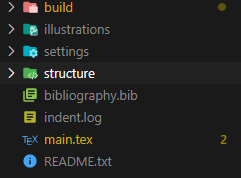
\includegraphics[width=0.5\linewidth]{illustrations/figures/example.png}
	\fonte{Autoria própria.}
\end{figure}

	\chapter{RELATO DO EXPERIMENTO}

\begin{figure}[H]
	\centering
	\caption{Engenheiro Eletricista}
	\label{fig:engenheiroeletricista}
	
\includegraphics[width=0.7\linewidth]{data/figures/EngenheiroEletricista}
	\fonte{\citeonline{ref:ufersa-caraubas}}
\end{figure}

A Engenharia Elétrica está presente na fabricação de praticamente todo produto manufaturado e daqueles que envolvem alta tecnologia, como satélites, aeronaves e produtos utilizados na automação industrial. Na verdade, esta engenharia se subdivide em várias áreas, como Eletrotécnica, Controle e Automação, Eletrônica, Microeletrônica e Telecomunicações.

O campo de atuação de um engenheiro eletricista é bastante amplo. Ele pode desenvolver atividades nas áreas de sistemas de geração, transmissão e distribuição de energia elétrica, controle e automação, instrumentação, sistemas eletrônicos analógicos e digitais, e projeto de circuitos integrados. Pode atuar no ramo das telecomunicações, em telefonia, antenas e propagação, na construção civil, na manutenção industrial, em informática, só para citar algumas possibilidades.

O profissional com formação em Engenharia Elétrica pode atuar não apenas em instituições privadas, mas também em órgãos governamentais, como agências reguladoras, secretarias, ministérios e autarquias em geral.
O mercado de trabalho está bem aquecido. As maiores oportunidades estão nas grandes e médias empresas multinacionais e em algumas nacionais. São crescentes também as possibilidades nas pequenas empresas nacionais que estão se modernizando para competir no mundo globalizado.

O engenheiro eletricista pode ainda seguir a carreira científica, atuando em centros de pesquisa e em universidades. Como em qualquer outra área de atuação, a preocupação com o ser humano e o meio ambiente é algo indispensável ao engenheiro formado atualmente.
	\chapter{CONCLUSÃO}

O curso de Graduação em Engenharia tem como perfil do formando egresso/profissional o engenheiro, com formação generalista, humanista, crítica e reflexiva, capacitado a absorver e desenvolver novas tecnologias, estimulando a sua atuação crítica e criativa na identificação e resolução de problemas, considerando seus aspectos políticos, econômicos, sociais, ambientais, culturais, com visão ética e humanística, em atendimento às demandas da sociedade.

	
	% seta os elementos pós-textuais
	\postextual
	\bibliography{settings/references}
\bibliographystyle{abntex2-alf} % Define o estilo ABNT para formatar a lista de referências
	
\end{document}
